\chapter{Ring of trust}
\section{Übersicht}

  Der Ring of Trust wird gebildet aus einer festen Reihenfolge der Zertifikate.
  Nach RFC 5280 wird diese Abfolge definiert. Grob zusammengefasst kann man sich
  die Abfolge der Zertifikate so vorstellen, dass Certificate Authority (kurz
  CA) einer der nächsten CA garantiert das sie vertrauenswürdig ist. Hierbei ist
  immer das ``Subject'' Feld des nächsten Zertifikats gleich dem Herausgeber des
  Vorherigen. So wird mithilfe des Privat keys von z.B. A das Zertifikat B
  verifiziert und B wurde mit dem Public key von Zertifikat A signiert. (siehe
  Abb. ~\ref{fig:certchain})\\

  \begin{figure}[!htb]
    \center 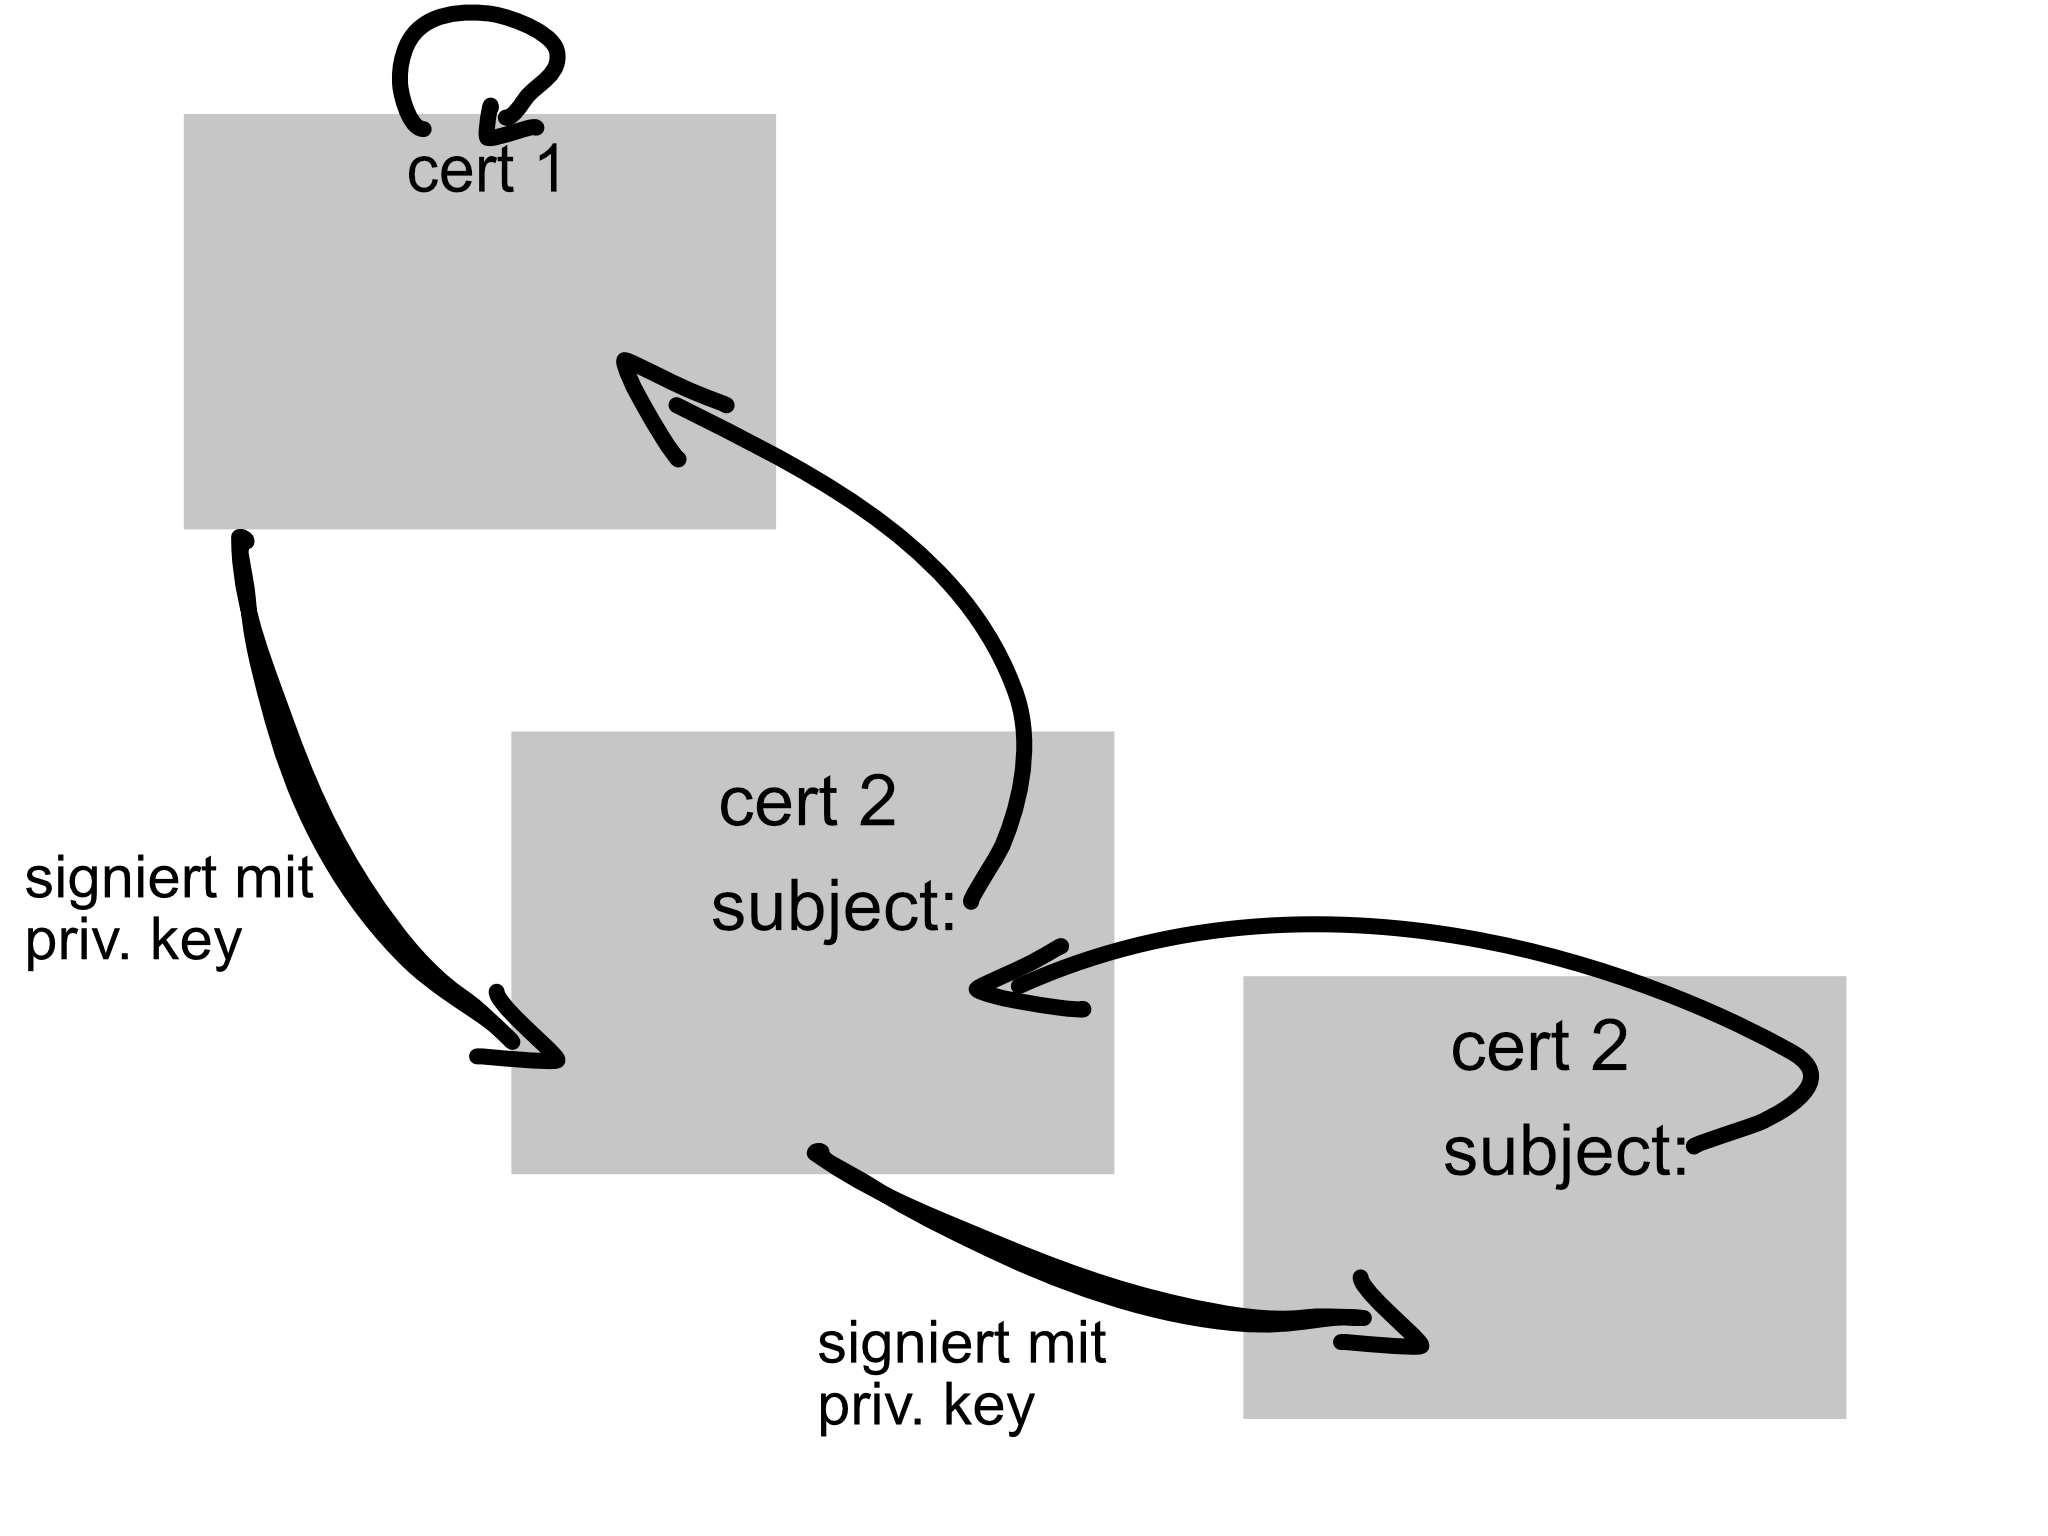
\includegraphics[scale=0.28]{images/rot.png}
    \caption{Zertifikatskette}
    \label{fig:certchain}
  \end{figure}

  \section{Root Zertifikate}
  Diese Kette löst sich so also von Zertifikat zu Zertifikat auf, bis ein s.g.
  Root Zertifikat erreicht wird. Dieses Zertifikat wurde mithilfe einer
  ``Vertrauenswürdigen Methode'' auf das Gerät übertragen. Die meisten
  Betriebsysteme haben solche Zertifikate vorinstalliert und Web-Browser haben
  auch meist eigene vertrauenswürdige Zertifikate. Diese Root Zertifikate sind
  der letzte Eintrag der Zertifikatskette und ihnen \textbf{muss} vertraut
  werden, da der Zertifikatsring hier endet.
  \pagebreak

  \section{Cross-Validierung}
  Damit CA's sich untereinander verifizieren können müssen Zertifikate kreuz
  validiert werden können. Dies wird gebraucht um zwei verschiedenen
  Verifizierungspfaden einen Weg zu schaffen Zertfikate untereinander zu
  vertrauen. Wie in Abb. ~\ref{fig:crossver} zu erkennen ist, wird für
  Kreuzvalidierung:
  \begin{enumerate}
  \item CA 1 gibt ein Zertifikat(cert 2.1) aus, was den Public key von CA 2 enthält.
  \item Nun kann mit dem nun User 2 mit seinem Zertifikat(cert 2.2) eine Vertrauenskette
    zu CA 1 über 2.1 aufbauen oder direkt zu CA 2 über cert 2
  \end{enumerate}


  \begin{figure}[!htb]
    \center 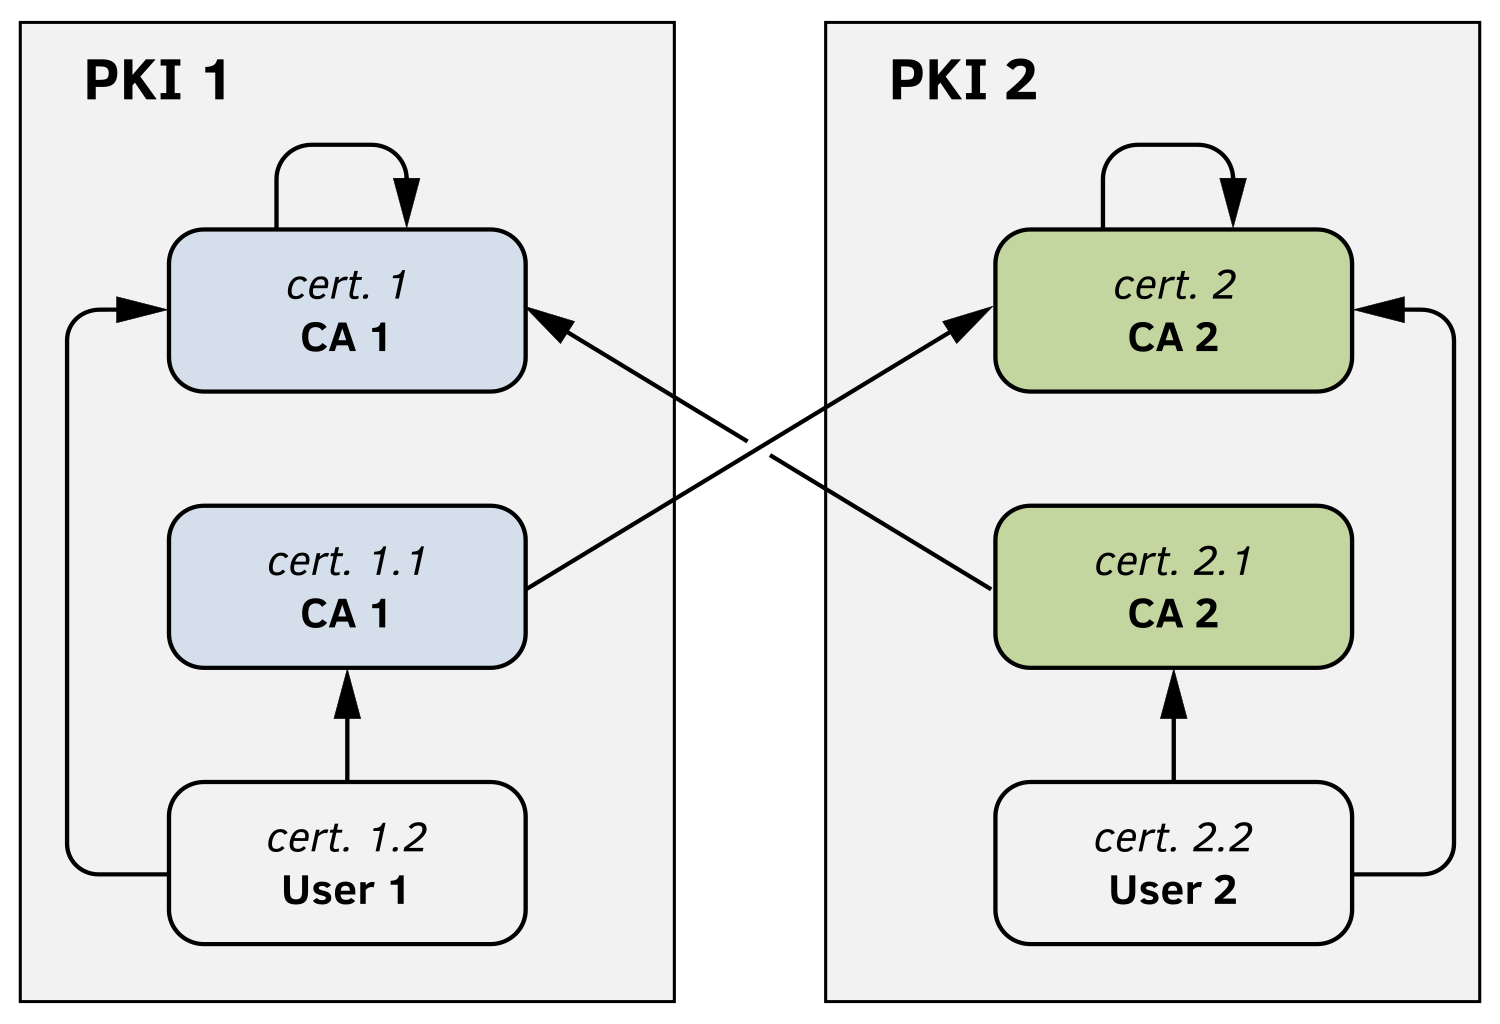
\includegraphics[scale=0.28]{images/ccd.png}
    \caption{Kreuzvalidierung}
    \label{fig:crossver}
  \end{figure}

  \section{CA Zertifikat Eneuerung}
  Um einen einfachen und leichten Übergang von auslaufenden CA Zertifikaten zu
  ermöglichen, kann die CA ein Zertifikat herausgeben, was den alten
  Public key enthält und mit dem neuen Private key signiert ist. Zeitgleich gibt
  die CA dann ein Zertifikat mit dem neuen Public key heraus, das mit dem alten
  Private key signiert ist